\documentclass[12pt]{report}

%====================== PACKAGES ======================


\usepackage{pgfgantt}

\usepackage[french]{babel}
\usepackage{tikz-uml}
\usepackage[french]{translator}
\usetikzlibrary{babel}
\usepackage[utf8x]{inputenc}
\usepackage[T1]{fontenc}
%pour gérer les positionnement d'images
\usepackage{float}
\usepackage{amsmath}
\usepackage{graphicx}

\usepackage{url}
%pour les informations sur un document compilé en PDF et les liens externes / internes
\usepackage{hyperref}
%pour la mise en page des tableaux
\usepackage{array}
\usepackage{tabularx}
%pour utiliser \floatbarrier
%\usepackage{placeins}
%\usepackage{floatrow}
%espacement entre les lignes
\usepackage{setspace}
%modifier la mise en page de l'abstract
\usepackage{abstract}
%police et mise en page (marges) du document
\usepackage[T1]{fontenc}
\usepackage[top=2cm, bottom=2cm, left=2cm, right=3.2cm]{geometry}
%Pour les galerie d'images
\usepackage{subfig}
\usepackage{listings}
\usepackage{scrextend}
\tikzumlset{fill class=orange!5, fill component=white, fill usecase=black!25, fill object=orange!25}
%====================== INFORMATION ET REGLES ======================

%rajouter les numérotation pour les \paragraphe et \subparagraphe
\setcounter{secnumdepth}{4}
\setcounter{tocdepth}{4}



%======================== DEBUT DU DOCUMENT ========================

\begin{document}

%régler l'espacement entre les lignes
\newcommand{\HRule}{\rule{\linewidth}{0.5mm}}

%page de garde
\begin{titlepage}
\begin{center}

% Upper part of the page. The '~' is needed because only works if a paragraph has started.

\includegraphics[width=0.35\textwidth]{./logo}~\\[1cm]

%\textsc{\LARGE Université ou Entreprise}\\[1.5cm]

\textsc{\Large }\\[0.5cm]

% Title
\HRule \\[0.4cm]

{\huge \bfseries \\ Découverte du framwork Apache OFBiz.
Dévéloppement d'une API HTTP, basé le sur style architectural REST et inégration dans un contexte de projet client. \\[0.4cm] }

\HRule \\[1.5cm]

% Author and supervisor
\begin{minipage}{0.4\textwidth}
\begin{flushleft} \large
\emph{Auteur:}\\
Artemiy \textsc{Rozovyk}\\

\end{flushleft}
\end{minipage}
\begin{minipage}{0.4\textwidth}
\begin{flushright} \large
\emph{Tuteur de stage:} \\
Mathieu \textsc{Lirzin}\\
\emph{Référent:} \\
Florent \textsc{Foucaud}
\end{flushright}
\end{minipage}

\vfill

% Bottom of the page
{\large \today}

\end{center}
\end{titlepage}
%ne pas numéroter cette page
\newpage
\tableofcontents
\newpage


\renewcommand{\abstractnamefont}{\normalfont\Large\bfseries}
%\renewcommand{\abstracttextfont}{\normalfont\Huge}

\renewcommand{\abstractname}{Remerciements}
\addcontentsline{toc}{chapter}{Remerciements}
\begin{abstract}
	Je tiens tout d'abord à remercier mon tuteur de stage, Mathieu Lirzin, pour les conseilles et les savoir-faire qu'il a partagé avec moi tout au long de mon stage. 
	\\
	
	De même, je remercie à Pierre Gaudin et à Antoine Ouvrard, pour leur collaboration et leur aide au cours des projets qu'on a pu développer ensemble. 
\\

	Enfin, merci à toute l’équipe de Néréide, pour leur accueil, leurs temps consacré à moi et leur bonne humeur constante.	
\end{abstract}

\newpage




%espacement entre les lignes d'un tableau
\renewcommand{\arraystretch}{1.5}

%====================== INCLUSION DES PARTIES ======================


%recommencer la numérotation des pages à "1"


\chapter{Introduction}

Intro\footnotemark\\
Intro2\footnotemark\\
%note en bas de page
\iffalse
\section{Sujet}

Bla(cf. fig. 1.1)\\

%inclusion d'une mage dans le document
\begin{figure}[!h]
\begin{center}
%taille de l'image en largeur
%remplacer "width" par "height" pour régler la hauteur
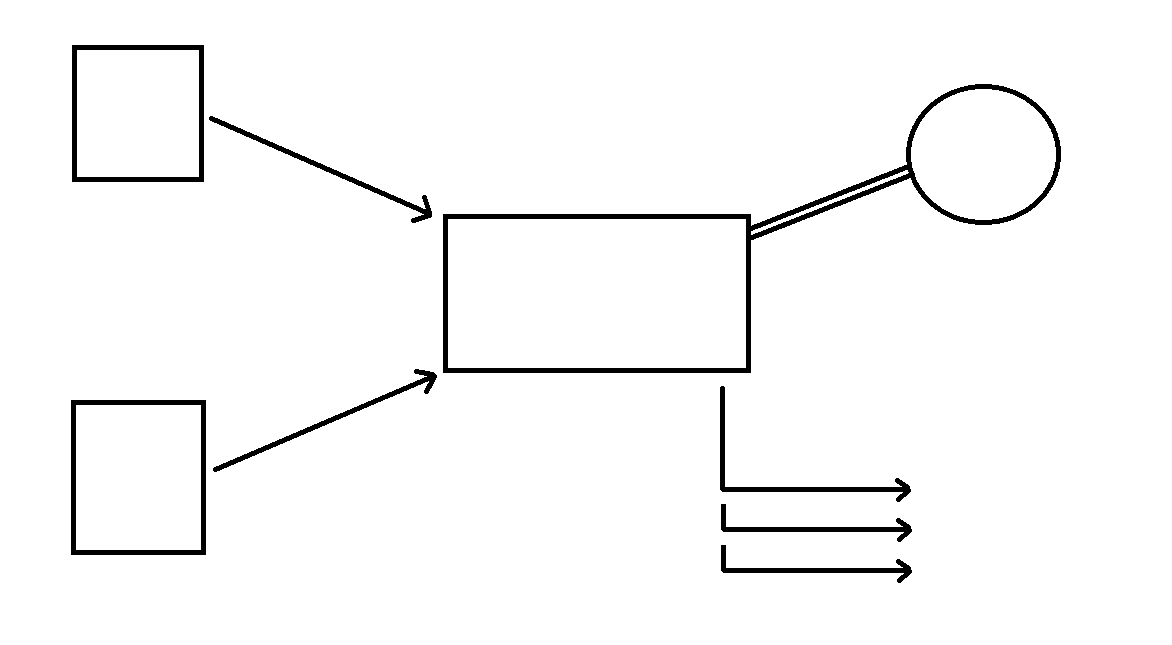
\includegraphics[width=15cm]{presentation/schema}
\end{center}
%légende de l'image
\caption{Schéma descriptif}
\end{figure}

%Contenu de la note précédemment marquée avec \footnotemark
\footnotetext{Note bas de page "intro"}

Bla
%retour à la ligne (alinea)

Bla\\
%saut de paragraphe

Bla

\newpage

\section{Problématique soulevée}

Bla

\begin{center}
Problématique du sujet
\end{center}

\section{Hypothèse de solution}

%Quoi :
Bla\\

Voici une liste :
\begin{itemize}
\item item 1;
\item item 2;
\item item 3;
\item item 4.
\end{itemize}

Bla\\

%Comment :
Bla

Bla\footnotemark\\

%Detail :
Bla(cf. ref. \cite{cite6}).
%citation référencé dans le document "bibliographie.bib" inclus à la fin du document
\fi
\footnotetext{Note bas de page "bla"}
\footnotetext{dog2}

\chapter{Contexte du stage}

Intro

\section{Entreprise}

\subsection{Presentation générale }
Néréide est une société de services en logiciels libres crée en 2004  SCOP SARL \\
parler de méthodes agiles. 
transparence interne totale ;
fonctionnement démocratique (SCOP, co-gérance tournante);
implication des salariés dans tous les domaines de décision ;
salaire unique


























\subsection{Domaine}
Retail
\subsection{Activité}
\label{activite}
Transparence libre entreprise \\


Integration(utilisation des briques en tant que telles) et
Dévéloppement spécifique (adaptation d'OFBIZ pour les besoins ) plugins propres à la logique métier. Pas de forfait(contrat doit etre rempli, l'entreprise s'engage à ce qu'il soit livré dans les tepms), mais la régie (sont payé au temps de travail et pas à condition de remplir un ... ).  Pareil avec Décath 6 pers font de la régie...
Administration système
\subsection{Projets}
Décathlon
 rfid store, interface pour les achteurs et producteurs, dev front pour le store specifique au lieu d'écrans OFBiz, communication avec des API...

Dejbox
\\
Dejbox est une société de la foodTech qui propose aux salariés d’entreprise de leur livrer des repas directement sur leur lieu de travail. L’ensemble des vente est réalisé au travers d’un site e-commerce par lequel le salarié commande un repas.

Le projet a pour objectif de mettre en œuvre un outil de type ERP afin de gérer la chaîne de réapprovisionnement en produit frais vendu en ligne. Il s’agit donc de créer un référentiel d’article et de fournisseur et de pouvoir saisir des commandes qui seront envoyées aux fournisseurs et réceptionnées suite à leur livraison. Enfin, il s’agit de mettre en place la sortie de stock en intégrant les consommations de produit provenant du site de vente en ligne.


....
Dépuis 2013 les dev remontantes à la communauté , parce que besoin de support,  divergence. moutons-acteur 






\newpage
\section{Framework OFBiz}
\subsection{Vue d'ensemble }
\emph{Open For Business (OFBiz)} est une suite d'applications pour la gestion de l'entreprise qui se base sur une architecture très couramment utilisé \emph{(MVC)} et qui implémente des composantes classiques de gestion des donnés, de logique métier, et de traitement spécialisé. 

On peut notamment distinguer les modules génériques destinées à la gestion des tâches communes à la plupart des entreprises, telles que la gestion des stocks, la comptabilité, la facturation et bien d'autres. Quant à leur structure, toutes les composantes sont étroitement liées entres elles, ce qui facilite la compréhension, l'utilisation et la personnalisation de ces dernières. 


En plus d'une architecture qui encourage la customisation, OFBiz est entièrement distribué en tant que \emph{open source software}\footnote{Logiciel libre sous licence \href{https://www.apache.org/licenses/LICENSE-2.0.html}{ASL2 (Apache License Version 2.0)} ce qui donne le droit de personnaliser, d'étendre, de restructurer et de vendre le système concerné. } ce qui le rend particulièrement intéressant car le logiciel développé à base d'OFBiz n'est pas soumis à la condition d'être libre comme c'est le cas de la licence GPL  \footnote{\href{http://www.gnu.org/licenses/gpl-3.0.html}{GNU General Public Licence}} par exemple.

\subsection{Architecture }
D'un point de vue purement technique OFBiz se base sur la plateforme Java ainsi que sur l'utilisation des DSL\footnote{Domaine specific language \emph{(Langages spé-cifiques au domaine)}} basés sur des grammaires écrites en XML (mettre la bib). En ce qui concerne la partie principale du framework, les échanges HTTP sont implémentes par une extension de la classe \verb=HTTPServlet= \cite{chan2017servlet} et la communication avec les bases de données se fait via l'API Java JDBC \cite{JDBC}.

Dans sa structure on distingue \emph{le framework}, \emph{les applications} et \emph{les plugins}. Le \emph{framework} comporte l'ensemble des outils et des mécanismes techniques, notamment en matière de  communication réseau et d'interaction entre les différentes applications.
Les principaux composants métier tels que la comptabilité, la gestion des stock, ou la facturation se trouvent dans la partie \emph{applications}. 
Finalement la notion du plugin correspond à une application spécifique qui repose sur des composantes générales: par exemple le plugin \emph{eCommerce} correspond à un boutique en ligne qui utilise des nombreuses  \emph{applications} comme \emph{la gestion du stock} ou \emph{la facturation}. 

\subsection{DSL XML}
L'une des particularités d'OFBiz ce sont des fichiers XML qui servent à déclarer entre autres
des routes HTTP, des pages de rendu appelés \emph{Écrans}, ainsi que des services. Le principe est de transformer des informations sous format XML facilement compréhensibles par le développeur, en objets Java correspondants. 


\definecolor{dollarbill}{rgb}{0.52, 0.73, 0.4}
\subsection{Container}
L'interface container représenté sur la figure \ref{container} permet de définir des objets qui correspondent à des processus qui peuvent être initialisés, démarrés et arrêtés. L'intérêt est de pouvoir lancer un daemon spécifique en parallèle de l'execution d'OFBiz comme c'est le cas de \verb|EntityDataLoadContainer| qui est responsable du chargement des données et leur mise à jour en cas de modification du modèle. Quand à \verb|TestRunContainer| il s'assure du lancement des testes unitaires grâce à un mécanisme spécifique du framework. 
\begin{figure}
	\centering
	\begin{tikzpicture}
	\umlinterface[scale=0.9,x=0,y=5]{Container}{}{
		\umlvirt{+ init(cmds : List<StartupCommand>, name : String,} \\
		\umlvirt{\hspace{1,1cm}config : String) : void} \\
		\umlvirt{+ start() : void} \\
		\umlvirt{+ stop() : void} \\
		\umlvirt{+ getName() : String}
	}
	\umlclass[ x=-5, y=-2]{EntityDataLoadContainer}{
		- name : String \\
		- module : String
	}{
		\umlvirt{+ getName() : String} \\
		\umlvirt{+ createDbConstraints(...) : void}\\
		\umlvirt{+ dropPrimaryKeys(...) : void}
	}
	\umlclass[ x=6, y=-2]{TestRunContainer}{
		- name : String \\
		- jsWrapper : JunitSuiteWrapper
	}{
		\umlvirt{+ getName() : String} \\
		\umlvirt{+ createJunitXmlListener(...) : JunitXmlListener} \\
		\umlvirt{+ logTestSuiteResults(...) : void} \\
	}

 \umldep[geometry=|-|, pos1=1.5, pos2=0.2 ,draw=dollarbill,  thick]{TestRunContainer}{Container}
 \umldep[geometry=|-|, pos1=1.5, pos2=0.2 ,draw=dollarbill,  thick]{EntityDataLoadContainer}{Container}
	\end{tikzpicture}
	
	
	\caption{Définition du type container}
	\label{container}
\end{figure}
\subsection{Composants}
Les éléments constitutifs de OFBIZ sont des composants. Un composant est un regroupement des containers, des entités, des services, des vues (\emph{Écrans}) et des applications Web.


L'exemple classique d'un composant est celui de \verb|webtools| qui assure la gestion technique de l'ensemble du système par l'administrateur via une application web, ce qui implique le fait que ce composant regroupe la plupart des éléments majeurs du framework.
Nous en tant que développeurs avons la possibilité de définir nos propres composants, notamment des \emph{plugins}. 
  


\subsection{Web applications}
Des composant OFBiz ne peuvent pas être accédés directement par les utilisateurs, ils servent simplement à organiser le framework en parties individuelles de chaque aspect de l'ERP afin de faciliter leur gestion. Les applications web \emph{(webapps)} sont destinées à fournir le front-end afin que les utilisateurs puissent interagir avec OFBiz. En ce qui concerne les routes HTTP, définis classiquement dans le fichier \verb|web.xml|, dans le cas de OFBiz leur gestion est délégué à un ficher \verb|controller.xml| qui à son tour associe des traitement spécifiques à chaque point d'entrée HTTP ainsi que la valeur de retour qui peut être une vue \emph{'un Écran)}, du type \verb|JSON| ou bien une redirection. Cela se fait au moyen d'une \verb|request-map| comme on peut voir sur \ref{reqmap}



\lstset{language=XML}
\begin{figure}
\begin{lstlisting}
<request-map uri="stock" method="get">
    <event type="service" invoke="getStock"/>
    <response name="success" type="view" value="stockScreen"/>
</request-map>
\end{lstlisting}
	\caption{Association d'un point d'entrée et d'une réponse}
\label{reqmap}
\end{figure}



\subsection{Entity engine}
Comme dans beaucoup d'autres frameworks, l'interaction avec les bases de données à une place principale dans le OFBiz. Le moteur d'entités (\emph{Entity engine}) se charge de la communication avec les  bases de données à travers les déclarations uniformes, c'est à dire qui changent pas peu importe le choix de l'outil externe de gestion.



\subsection{Service engine}
Les services web assurent les échanges d'information être les applications, communément via protocole \verb| HTTP|.   
Les services OFBiz fonctionnent dans une architecture orientée service (SOA). Non seulement ces services ont une capacité d'évoquer les autres intérieurement, mais peuvent aussi être appelés par une application extérieure en utilisant des protocoles d'échange d'information telles que \verb|SOAP|. 

Les services OFBiz sont appelées en passant un contexte \footnote{Définis souvent dans les paramètres de la requête \verb|HTTP| } et retournent une réponse parmi celles conventionnellement nommés: \emph{"success"}, comme on peut voir dans  \ref{reqmap} , \emph{"error"} ou \emph{"failure"} ainsi que l'ensemble des données retournées par le service. 

On peut voir la définition d'un service sur \ref{servicedef} , qui montre notamment les attributs attendu par le services qui sont défini de deux manières: En utilisant le mécanisme de \verb|auto-attributes| qui génère des attributs en entrée (de paramètre \verb|IN|) à partir de l'ensemble des clés primaires de l'entité \verb|Stock|. L'autre manière de faire est de rajouter des attributs manuellement comme on peut le voir dans la suite de l'exemple. 


\begin{figure}
\begin{lstlisting}
<service name="getStock" engine="entity-auto" default-entity-name="Stock">
  <auto-attributes include="pk" mode="IN" optional="false"/>
  <attribute name="authKey" type="String" mode="IN" optional="true"/>
  <attribute name="stockList" type="String" mode="OUT" optional="true"/>
</service>
\end{lstlisting}
\caption{Association d'un point d'entrée et d'une réponse}
\label{servicedef}
\end{figure}


\subsection{Screen engine}
\subsection{Fonctionnel métier}

\newpage
\section{Sujet de stage }



\subsection{API REST au sein d'OFBiz}

Jira

 
\chapter{Travail réalisé}


\section{Aperçu général}
Voici la chronologie du travail réalisé en entreprise.\\
\ganttset{%
	calendar week text={%
		\pgfcalendarmonthshortname{\startmonth}~\startday%
	}%
}
\newganttlinktype{f-m}{
	\ganttsetstartanchor{on right=1}
	\ganttsetendanchor{on left=0}
	\draw[/pgfgantt/link]
	([xshift=-.2pt]\xLeft, \yUpper) --       % xshift to fit arrow
	node[pos=.5, /pgfgantt/link label node] {\ganttlinklabel} 
	(\xRight, \yLower);
}


%vgrid={*1{blue!30},
%	*6{black,dotted},
%	*1{red!30},
%	*2{black,dotted},
%	*1{blue!30},
%	*{34}{black,dotted},
%	*1{green!30},
%	*1{red!30},
%	*{10}{black,dotted},
%	*1{green!30}},
\setganttlinklabel{f-m}{}

\begin{ganttchart}[
	hgrid,
	vgrid,
	x unit=2.9mm,
	time slot format=isodate,
	inline,
	bar/.append style={fill=blue!37},
	group/.append style={draw=black, fill=black!50},
	milestone/.append style={fill=green, rounded corners=6pt,scale=2},
	milestone inline label node/.append style={right=1mm},
	]{2019-03-28}{2019-05-25}
	\gantttitlecalendar{year, month=name, week} \\
	\ganttgroup{Analyse des besoins}{2019-03-29}{2019-04-7}\\
	\ganttgroup{Réalisation technique}{2019-04-5}{2019-05-13}\\
	\ganttgroup{Maintenance}{2019-05-13}{2019-05-24} \\
	\ganttbar{OFBiz}{2019-04-01}{2019-04-11}\\
	\ganttbar[
	bar/.append style={ fill=red!50
	}]{REST}{2019-04-08}{2019-04-28} \\
	\ganttbar[
	bar/.append style={ fill=orange!50
	}]{Entitymaint}{2019-04-20}{2019-05-12} \\
	
	\ganttmilestone{Preuve de concept}{2019-05-12}] \\
	\ganttbar[
	bar/.append style={ fill=purple!40, dashed
	}]{Revue de code}{2019-05-13}{2019-05-23} \\
	\ganttlink{elem3}{elem4}
	\ganttlink{elem4}{elem5}
	\ganttlink[link type=f-m]{elem5}{elem6}
	\ganttlink[link type=dr]{elem4}{elem6}
	\ganttlink[link type=f-m]{elem6}{elem7}
\end{ganttchart}

\newpage









\section{Environnement}

\subsection{Installation de l'environnement}
Avant tout, mon intégration a commencé par l'installation du poste de travail suivi par une discussion sur le choix de distribution Linux \footnote{Une question qui a, apparemment, beaucoup d'importance.} , la configuration des outils utilisés par l'entreprise ainsi que par la mise en place des accès aux ressources internes \footnote{Contenaient, à mon avis, des information sensibles, mais cela s'explique par le principe de transparence \ref{activite} }



\subsection{Conventions}
\subsection{Formation développeur générale}
\subsection{Jira}
\subsection{Approfondissement de Git }
\subsection{Découverte de communauté libre Apache}

\newpage
\section{Prise en main d'OFBiz}

\subsection{Premier plugin}

\subsection{Projets existants et leur structure}
\subsubsection{Décathlon}
RFID et tout ça
\subsubsection{Dejbox}
Pierre et Antoine ont tout géré 

\subsection{Problématique vis-à-vis du développement}
What is "fonctionnel"

\newpage

\section{Analyse de l'existant}
\subsection{ControlServlet}
\subsection{Mécanisme de résolution des URI}
\subsection{Filtres}
Delegateur et Dispatcher


\newpage

\section{Analyse des besoins et attentes de la maîtrise d'ouvrage}
\subsection{Structure générale des application web}
Les enjeux, les problématiques les solutions, *COURS MAURIZIO*
\subsection{API en cours}
RPC
\subsection{Controleur}
<request-map>...
\subsection{Besoins d'évolution}
Avenir
*Discussion communautaire*
\subsection{Representational state transfer}
\subsubsection{Histoire}
Roy Fielding
\subsubsection{Principe}
*Détailles du cours de Maurizio: idempotence, navigabilité par hyperlink, 
notion de ressource etc.
\subsubsection{Avantages}
\subsubsection{Examples d'API du style REST}
API REST de Twitter, SoundCloud, Wiktionnaire,\\
les différences entre la définition de Roy Fielding et l'implémentation de ces dernières

\subsection{Implementations existantes}
\subsubsection{Camel}
\subsubsection{JAX-RS}
Tentative d'intégration ---\\
ServletJaxRS fonctionnelle\\
Particularités techniques (annotations) \\
Conflit politique car n'est pas dans le même esprit de l'existant.\\



\newpage

\section{Réalisations techniques}

\subsection{Librairie CXF}
Problèmatique avec les dépendances supplementaires: 
Tika contient déjà le CXF
\subsection{Choix vers URITemplate}
description de classe
\subsection{\textit{OverrideView()} et le conflit avec les URI segmentées}
\subsection{Choix d'intégration en parallèle avec le système existant }
\subsection{Nouveau contrôleur}
\subsubsection{Compromis pour les conflits d'URI}

\subsection{Modification de la partie "Administration: gestion des entités"  (entitymaint)  }
\subsubsection{Choix de la partie illustrative}
\subsubsection{PUT vs POST}
\subsubsection{Clés composées}
\subsubsection{Formulaires génériques }
Create update dans un même formulaire.
\subsection{Stateless}
\subsubsection{Les réalisation par la communauté}

Jaques Le Roux Token en gardant la session.
\subsection{RESTClient pour la communauté}
\subsubsection{Généralisation de code}
\subsubsection{Correction d'incohérences}



\iffalse
\section{Besoins fonctionnels}

Après une analyse des besoins fonctionnels du projet, nous avons défini deux sous catégories. D'un côté, les besoins [...], de l'autre, les besoins [...].

\subsection{Sous-partie 1}

Bla

\subsection{Sous-partie 2}

Bla

\newpage

\section{Besoins non-fonctionnels}

Comme précédemment, nous avons choisi de distinguer deux catégories pour les besoins non-fonctionnels. D'une part, nous avons les besoins non-fonctionnels pour les [...], et d'autre part ceux pour [...]. Nous avons aussi pris en compte les contraintes de développement, que nous détaillerons à la fin de cette partie.

\subsection{Sous-partie 1}

Bla\\

Aperçu du rendu souhaité :

\begin{figure}[!h]
\begin{center}
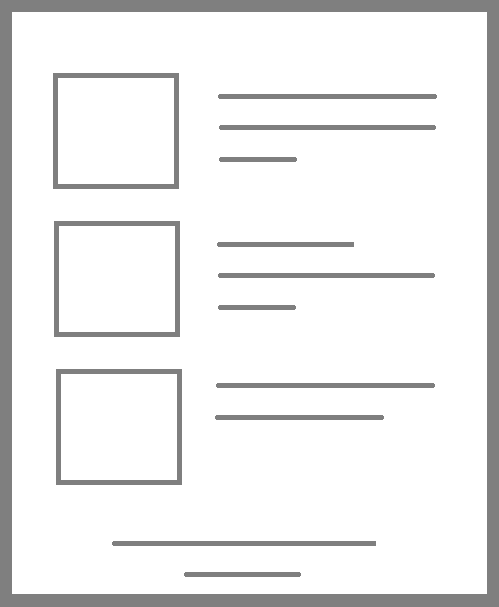
\includegraphics[height=10cm]{besoins/rendu}
\end{center}
\caption{Rendu attendu}
\end{figure}

\subsection{Sous-partie 2}

Bla

\newpage

\section{Développement}

Intro

\subsection{Tâches}

Bla\\


%tableau à taille fixée sur certaines colonnes (param sur la ligne \begin{tabularx}, voir wiki pour plus d'info sur la syntaxe
\begin{figure}[!h]
\begin{center}
\begin{tabularx}{17cm}{|c|p{6cm}|X|}
  \hline
  Priorité & Nom & Raison\\
  \hline
  1 & Tache 1 & Doit être vérifié en premier car sinon [...] \tabularnewline
  2 & Tache 2 & On doit pouvoir [...] \tabularnewline
  3 & Tache 3 & Comme les principales fonctionnalités permettant de tester sont opérationnelles, nous pouvons passer à cette tâche. \tabularnewline
  4 & Tache 4 & Parce que [...] \tabularnewline
  5 & Tache 5 & La tache 5 fait partie des principales [...]. \tabularnewline
  6 & Tache 6 & Dernière fonctionnalité essentielle à mettre en place. \tabularnewline
  7 & Tache 7 & Non-essentiel, mais apporterait un plus au projet. \tabularnewline
  8 & Tache 8 & Non-essentiel, mais apporterait un plus au projet. \tabularnewline
  \hline
\end{tabularx}
\end{center}
\caption{Tableau récapitulatif des tâches}
\end{figure}

\subsection{Tests}

Bla\\

\begin{figure}[!h]
\begin{center}
\begin{tabularx}{17cm}{|p{6cm}|X|}
  \hline
  Fonctionnalité & Test\\
  \hline
  Fonction 1 & Quand [...], vérifier [...]. \tabularnewline
  & Et quand [...], vérifier [...]. \tabularnewline
  Fonction 2 & Vérifier [...]. \tabularnewline
  Fonction 3 & Vérifier [...]. \tabularnewline
  Fonction 4 & Avoir [...]. \tabularnewline
  Fonction 5 & Accéder à [...]. \tabularnewline
   & Vérifier que [...]. \tabularnewline
  Fonction 6 & Accéder à [...]. \tabularnewline
   & Et vérifier [...]. \tabularnewline
  Fonction 7 & Installer [...]. \tabularnewline
   & Vérifier [...]. \tabularnewline
  Fonction 8 & Compter [...]. \tabularnewline
  \hline
\end{tabularx}
\end{center}
\caption{Tableau récapitulatif des tests}
\end{figure}
\fi

\chapter{Conclusion}
\ganttset{%
	calendar week text={%
		\pgfcalendarmonthshortname{\startmonth}~\startday%
	}%
}
\newganttlinktype{f-m}{
	\ganttsetstartanchor{on right=1}
	\ganttsetendanchor{on left=0}
	\draw[/pgfgantt/link]
	([xshift=-.2pt]\xLeft, \yUpper) --       % xshift to fit arrow
	node[pos=.5, /pgfgantt/link label node] {\ganttlinklabel} 
	(\xRight, \yLower);
}
\setganttlinklabel{f-m}{}

	\begin{ganttchart}[
		hgrid,
		vgrid={*1{blue!30},
			 *6{black,dotted},
			 *1{red!30},
			 *2{black,dotted},
			 *1{blue!30},
			 *{34}{black,dotted},
		 	 *1{green!30},
	 	 	 *1{red!30},
 	 	 	 *{10}{black,dotted},
  	 	 	 *1{green!30}},
		x unit=3mm,
		time slot format=isodate,
		inline,
		bar/.append style={fill=blue!37},
	    group/.append style={draw=black, fill=black!50},
		milestone/.append style={fill=green, rounded corners=6pt,scale=2},
		milestone inline label node/.append style={right=1mm},
	]{2019-03-28}{2019-05-25}
	\gantttitlecalendar{year, month=name, week} \\
	\ganttgroup{Analyse des besoins}{2019-03-29}{2019-04-7}\\
	\ganttgroup{Réalisation technique}{2019-04-5}{2019-05-13}\\
	\ganttgroup{Maintenance}{2019-05-13}{2019-05-24} \\
	\ganttbar{OFBiz}{2019-04-01}{2019-04-11}\\
	\ganttbar[
	bar/.append style={ fill=red!50
	}]{REST}{2019-04-08}{2019-04-28} \\
	\ganttbar[
	bar/.append style={ fill=orange!50
	}]{Entitymaint}{2019-04-20}{2019-05-12} \\

	\ganttmilestone{Preuve de concept}{2019-05-12}] \\
	\ganttbar[
	bar/.append style={ fill=purple!40, dashed
	}]{Revue de code}{2019-05-13}{2019-05-23} \\
	\ganttlink{elem3}{elem4}
	\ganttlink{elem4}{elem5}
	\ganttlink[link type=f-m]{elem5}{elem6}
	\ganttlink[link type=dr]{elem4}{elem6}
	\ganttlink[link type=f-m]{elem6}{elem7}
	\end{ganttchart}

\newpage

%récupérer les citation avec "/footnotemark"
\nocite{*}

%choix du style de la biblio
\bibliographystyle{plain}
%inclusion de la biblio
\bibliography{bibliographie.bib}
%voir wiki pour plus d'information sur la syntaxe des entrées d'une bibliographie

\end{document}